\section{Metodo di Newton}
\label{sec:metodoDiNewton}

\begin{exercise}
Implementare il metodo di newton ed applicarlo alla funzione \emph{chordConvergenceFunction},
con innesco iniziale $x_{0} = 5.3$, una tollerenza assoluta e relativa
$tol_{X} = rTol_{X} = 10^{-14}$ ed un numero massimo di iterazioni
$i_{max} = 10^{5}$.
\end{exercise}
Per l'implementazione del codice vedere \nameref{subsec:chordMethodLinearCriteria}.
\begin{lstlisting}
octave:112> [x, i, ascisse] =
chordMethodLinearCriteria('chordConvergenceFunction','chordConvergenceFunctionDerivative',5.3, 1e5, 1e-14, 1e-14) 
x =  1.78658833723778e+00
i =  9.40000000000000e+01
ascisse = [too long to report here]
octave:113> xSingleZero = min(ascisse)-1:0.1:max(ascisse)+1
octave:114> ySingleZero = invokeDelegate('chordConvergenceFunction', xSingleZero)
octave:115> [prepX, prepY] = prepareForPlottingMethodSegments(ascisse, 'invokeDelegate', 'chordConvergenceFunction')
octave:116> plot(xSingleZero, ySingleZero, "c", ascisse, invokeDelegate('chordConvergenceFunction', ascisse), "b+", prepX, prepY, "r")
octave:117> axis([1.3, 5.5, -5, 20])
octave:118> grid
octave:119> print 'chordPlotOutput.tex' '-dTex' '-S800, 600'
\end{lstlisting}
Si raggiunge la tolleranza richiesta in 94 passi. Questo l'output del comando
\emph{octave:119}:
\begin{center}
% GNUPLOT: LaTeX picture with Postscript
\begingroup
  \makeatletter
  \providecommand\color[2][]{%
    \GenericError{(gnuplot) \space\space\space\@spaces}{%
      Package color not loaded in conjunction with
      terminal option `colourtext'%
    }{See the gnuplot documentation for explanation.%
    }{Either use 'blacktext' in gnuplot or load the package
      color.sty in LaTeX.}%
    \renewcommand\color[2][]{}%
  }%
  \providecommand\includegraphics[2][]{%
    \GenericError{(gnuplot) \space\space\space\@spaces}{%
      Package graphicx or graphics not loaded%
    }{See the gnuplot documentation for explanation.%
    }{The gnuplot epslatex terminal needs graphicx.sty or graphics.sty.}%
    \renewcommand\includegraphics[2][]{}%
  }%
  \providecommand\rotatebox[2]{#2}%
  \@ifundefined{ifGPcolor}{%
    \newif\ifGPcolor
    \GPcolortrue
  }{}%
  \@ifundefined{ifGPblacktext}{%
    \newif\ifGPblacktext
    \GPblacktexttrue
  }{}%
  % define a \g@addto@macro without @ in the name:
  \let\gplgaddtomacro\g@addto@macro
  % define empty templates for all commands taking text:
  \gdef\gplbacktext{}%
  \gdef\gplfronttext{}%
  \makeatother
  \ifGPblacktext
    % no textcolor at all
    \def\colorrgb#1{}%
    \def\colorgray#1{}%
  \else
    % gray or color?
    \ifGPcolor
      \def\colorrgb#1{\color[rgb]{#1}}%
      \def\colorgray#1{\color[gray]{#1}}%
      \expandafter\def\csname LTw\endcsname{\color{white}}%
      \expandafter\def\csname LTb\endcsname{\color{black}}%
      \expandafter\def\csname LTa\endcsname{\color{black}}%
      \expandafter\def\csname LT0\endcsname{\color[rgb]{1,0,0}}%
      \expandafter\def\csname LT1\endcsname{\color[rgb]{0,1,0}}%
      \expandafter\def\csname LT2\endcsname{\color[rgb]{0,0,1}}%
      \expandafter\def\csname LT3\endcsname{\color[rgb]{1,0,1}}%
      \expandafter\def\csname LT4\endcsname{\color[rgb]{0,1,1}}%
      \expandafter\def\csname LT5\endcsname{\color[rgb]{1,1,0}}%
      \expandafter\def\csname LT6\endcsname{\color[rgb]{0,0,0}}%
      \expandafter\def\csname LT7\endcsname{\color[rgb]{1,0.3,0}}%
      \expandafter\def\csname LT8\endcsname{\color[rgb]{0.5,0.5,0.5}}%
    \else
      % gray
      \def\colorrgb#1{\color{black}}%
      \def\colorgray#1{\color[gray]{#1}}%
      \expandafter\def\csname LTw\endcsname{\color{white}}%
      \expandafter\def\csname LTb\endcsname{\color{black}}%
      \expandafter\def\csname LTa\endcsname{\color{black}}%
      \expandafter\def\csname LT0\endcsname{\color{black}}%
      \expandafter\def\csname LT1\endcsname{\color{black}}%
      \expandafter\def\csname LT2\endcsname{\color{black}}%
      \expandafter\def\csname LT3\endcsname{\color{black}}%
      \expandafter\def\csname LT4\endcsname{\color{black}}%
      \expandafter\def\csname LT5\endcsname{\color{black}}%
      \expandafter\def\csname LT6\endcsname{\color{black}}%
      \expandafter\def\csname LT7\endcsname{\color{black}}%
      \expandafter\def\csname LT8\endcsname{\color{black}}%
    \fi
  \fi
  \setlength{\unitlength}{0.0500bp}%
  \begin{picture}(7680.00,5760.00)%
    \gplgaddtomacro\gplbacktext{%
      \colorrgb{0.00,0.00,0.00}%
      \put(866,634){\makebox(0,0)[r]{\strut{}-5}}%
      \colorrgb{0.00,0.00,0.00}%
      \put(866,1573){\makebox(0,0)[r]{\strut{}0}}%
      \colorrgb{0.00,0.00,0.00}%
      \put(866,2511){\makebox(0,0)[r]{\strut{}5}}%
      \colorrgb{0.00,0.00,0.00}%
      \put(866,3450){\makebox(0,0)[r]{\strut{}10}}%
      \colorrgb{0.00,0.00,0.00}%
      \put(866,4388){\makebox(0,0)[r]{\strut{}15}}%
      \colorrgb{0.00,0.00,0.00}%
      \put(866,5327){\makebox(0,0)[r]{\strut{}20}}%
      \colorrgb{0.00,0.00,0.00}%
      \put(1281,414){\makebox(0,0){\strut{}1.5}}%
      \colorrgb{0.00,0.00,0.00}%
      \put(1990,414){\makebox(0,0){\strut{}2}}%
      \colorrgb{0.00,0.00,0.00}%
      \put(2699,414){\makebox(0,0){\strut{}2.5}}%
      \colorrgb{0.00,0.00,0.00}%
      \put(3407,414){\makebox(0,0){\strut{}3}}%
      \colorrgb{0.00,0.00,0.00}%
      \put(4116,414){\makebox(0,0){\strut{}3.5}}%
      \colorrgb{0.00,0.00,0.00}%
      \put(4824,414){\makebox(0,0){\strut{}4}}%
      \colorrgb{0.00,0.00,0.00}%
      \put(5533,414){\makebox(0,0){\strut{}4.5}}%
      \colorrgb{0.00,0.00,0.00}%
      \put(6241,414){\makebox(0,0){\strut{}5}}%
      \colorrgb{0.00,0.00,0.00}%
      \put(6950,414){\makebox(0,0){\strut{}5.5}}%
    }%
    \gplgaddtomacro\gplfronttext{%
    }%
    \gplbacktext
    \put(0,0){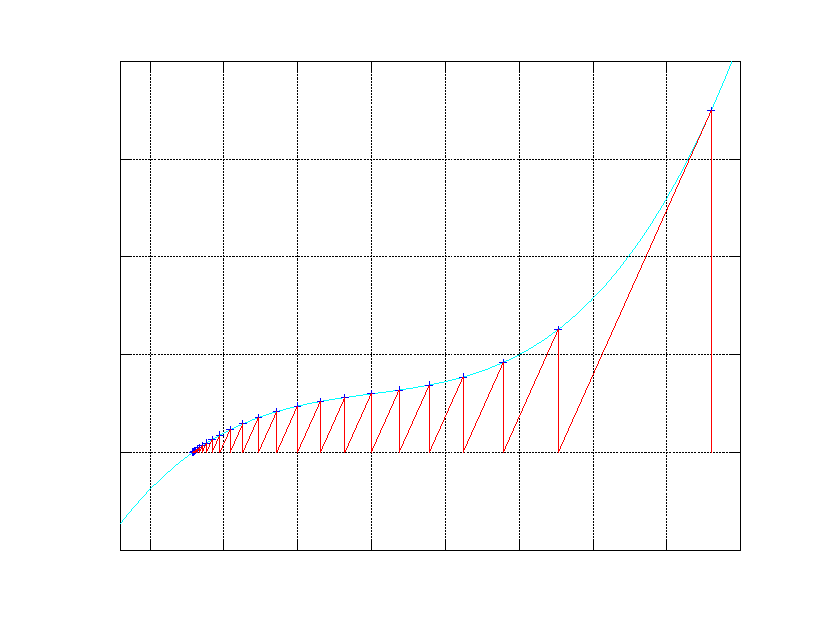
\includegraphics{RadiciEquazione/quasiNewton/chordPlotOutput}}%
    \gplfronttext
  \end{picture}%
\endgroup

\end{center}


\begin{exercise}
Applicare il metodo delle corde in riferimentoa all'esercizio
\ref{exercise:newtonLoopStartingPoint} 
Usare una tollerenza assoluta e relativa
$tol_{X} = rTol_{X} = 10^{-14}$ ed un numero massimo di iterazioni
$i_{max} = 10^{5}$ e punto di innesco $x_{0} = 10$.
\end{exercise}
Per l'implementazione del codice vedere \nameref{subsec:chordMethodLinearCriteria}.
\begin{lstlisting}
octave:112> [x, i, ascisse] = chordMethodLinearCriteria('functionNewtonRecursion','functionNewtonRecursionDerivative',10,1e5, 1e-10, 1e-10)
x =  2.23606797759911e+00
i =  6.67000000000000e+02
ascisse = [too long to report here]
octave:113> xSingleZero = min(ascisse)-1:0.1:max(ascisse)+1
octave:114> ySingleZero = invokeDelegate('functionNewtonRecursion', xSingleZero)
octave:115> [prepX, prepY] = prepareForPlottingMethodSegments(ascisse, 'invokeDelegate', 'functionNewtonRecursion')
octave:116> plot(xSingleZero, ySingleZero, "c", ascisse, invokeDelegate('functionNewtonRecursion', ascisse), "b+", prepX, prepY, "r")
octave:117> axis([2, 5, -25, 100])
octave:118> grid
octave:119> print 'chordNewtonRecursionPlotOutput.tex' '-dTex' '-S800, 600'
\end{lstlisting}
Si raggiunge la tolleranza richiesta in 667 passi. Questo l'output del comando
\emph{octave:119}:
\begin{center}
% GNUPLOT: LaTeX picture with Postscript
\begingroup
  \makeatletter
  \providecommand\color[2][]{%
    \GenericError{(gnuplot) \space\space\space\@spaces}{%
      Package color not loaded in conjunction with
      terminal option `colourtext'%
    }{See the gnuplot documentation for explanation.%
    }{Either use 'blacktext' in gnuplot or load the package
      color.sty in LaTeX.}%
    \renewcommand\color[2][]{}%
  }%
  \providecommand\includegraphics[2][]{%
    \GenericError{(gnuplot) \space\space\space\@spaces}{%
      Package graphicx or graphics not loaded%
    }{See the gnuplot documentation for explanation.%
    }{The gnuplot epslatex terminal needs graphicx.sty or graphics.sty.}%
    \renewcommand\includegraphics[2][]{}%
  }%
  \providecommand\rotatebox[2]{#2}%
  \@ifundefined{ifGPcolor}{%
    \newif\ifGPcolor
    \GPcolortrue
  }{}%
  \@ifundefined{ifGPblacktext}{%
    \newif\ifGPblacktext
    \GPblacktexttrue
  }{}%
  % define a \g@addto@macro without @ in the name:
  \let\gplgaddtomacro\g@addto@macro
  % define empty templates for all commands taking text:
  \gdef\gplbacktext{}%
  \gdef\gplfronttext{}%
  \makeatother
  \ifGPblacktext
    % no textcolor at all
    \def\colorrgb#1{}%
    \def\colorgray#1{}%
  \else
    % gray or color?
    \ifGPcolor
      \def\colorrgb#1{\color[rgb]{#1}}%
      \def\colorgray#1{\color[gray]{#1}}%
      \expandafter\def\csname LTw\endcsname{\color{white}}%
      \expandafter\def\csname LTb\endcsname{\color{black}}%
      \expandafter\def\csname LTa\endcsname{\color{black}}%
      \expandafter\def\csname LT0\endcsname{\color[rgb]{1,0,0}}%
      \expandafter\def\csname LT1\endcsname{\color[rgb]{0,1,0}}%
      \expandafter\def\csname LT2\endcsname{\color[rgb]{0,0,1}}%
      \expandafter\def\csname LT3\endcsname{\color[rgb]{1,0,1}}%
      \expandafter\def\csname LT4\endcsname{\color[rgb]{0,1,1}}%
      \expandafter\def\csname LT5\endcsname{\color[rgb]{1,1,0}}%
      \expandafter\def\csname LT6\endcsname{\color[rgb]{0,0,0}}%
      \expandafter\def\csname LT7\endcsname{\color[rgb]{1,0.3,0}}%
      \expandafter\def\csname LT8\endcsname{\color[rgb]{0.5,0.5,0.5}}%
    \else
      % gray
      \def\colorrgb#1{\color{black}}%
      \def\colorgray#1{\color[gray]{#1}}%
      \expandafter\def\csname LTw\endcsname{\color{white}}%
      \expandafter\def\csname LTb\endcsname{\color{black}}%
      \expandafter\def\csname LTa\endcsname{\color{black}}%
      \expandafter\def\csname LT0\endcsname{\color{black}}%
      \expandafter\def\csname LT1\endcsname{\color{black}}%
      \expandafter\def\csname LT2\endcsname{\color{black}}%
      \expandafter\def\csname LT3\endcsname{\color{black}}%
      \expandafter\def\csname LT4\endcsname{\color{black}}%
      \expandafter\def\csname LT5\endcsname{\color{black}}%
      \expandafter\def\csname LT6\endcsname{\color{black}}%
      \expandafter\def\csname LT7\endcsname{\color{black}}%
      \expandafter\def\csname LT8\endcsname{\color{black}}%
    \fi
  \fi
  \setlength{\unitlength}{0.0500bp}%
  \begin{picture}(7680.00,5760.00)%
    \gplgaddtomacro\gplbacktext{%
      \colorrgb{0.00,0.00,0.00}%
      \put(866,822){\makebox(0,0)[r]{\strut{}-20}}%
      \colorrgb{0.00,0.00,0.00}%
      \put(866,1573){\makebox(0,0)[r]{\strut{}0}}%
      \colorrgb{0.00,0.00,0.00}%
      \put(866,2323){\makebox(0,0)[r]{\strut{}20}}%
      \colorrgb{0.00,0.00,0.00}%
      \put(866,3074){\makebox(0,0)[r]{\strut{}40}}%
      \colorrgb{0.00,0.00,0.00}%
      \put(866,3825){\makebox(0,0)[r]{\strut{}60}}%
      \colorrgb{0.00,0.00,0.00}%
      \put(866,4576){\makebox(0,0)[r]{\strut{}80}}%
      \colorrgb{0.00,0.00,0.00}%
      \put(866,5327){\makebox(0,0)[r]{\strut{}100}}%
      \colorrgb{0.00,0.00,0.00}%
      \put(998,414){\makebox(0,0){\strut{}2}}%
      \colorrgb{0.00,0.00,0.00}%
      \put(1990,414){\makebox(0,0){\strut{}2.5}}%
      \colorrgb{0.00,0.00,0.00}%
      \put(2982,414){\makebox(0,0){\strut{}3}}%
      \colorrgb{0.00,0.00,0.00}%
      \put(3974,414){\makebox(0,0){\strut{}3.5}}%
      \colorrgb{0.00,0.00,0.00}%
      \put(4966,414){\makebox(0,0){\strut{}4}}%
      \colorrgb{0.00,0.00,0.00}%
      \put(5958,414){\makebox(0,0){\strut{}4.5}}%
      \colorrgb{0.00,0.00,0.00}%
      \put(6950,414){\makebox(0,0){\strut{}5}}%
    }%
    \gplgaddtomacro\gplfronttext{%
    }%
    \gplbacktext
    \put(0,0){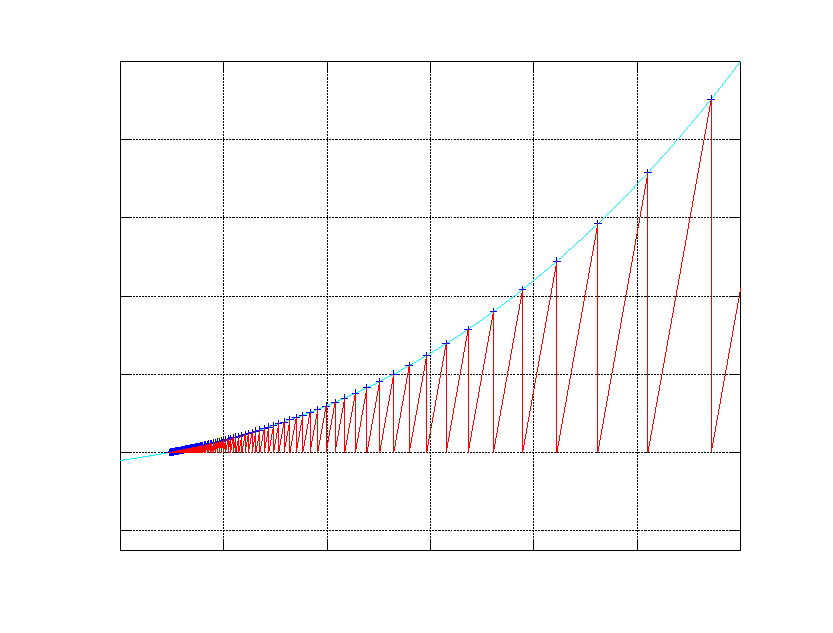
\includegraphics{RadiciEquazione/quasiNewton/chordNewtonRecursionPlotOutput}}%
    \gplfronttext
  \end{picture}%
\endgroup

\end{center}

Se invece voglio trovare la soluzione negativa:
\begin{lstlisting}
octave:112> [x, i, ascisse] = chordMethodLinearCriteria('functionNewtonRecursion','functionNewtonRecursionDerivative',-5,1e5, 1e-5, 1e-5)
i =  7.30000000000000e+01
ascisse = [too long to report here]
octave:113> xSingleZero = min(ascisse)-1:0.1:max(ascisse)+1
octave:114> ySingleZero = invokeDelegate('functionNewtonRecursion', xSingleZero)
octave:115> [prepX, prepY] = prepareForPlottingMethodSegments(ascisse, 'invokeDelegate', 'functionNewtonRecursion')
octave:116> plot(xSingleZero, ySingleZero, "c", ascisse, invokeDelegate('functionNewtonRecursion', ascisse), "b+", prepX, prepY, "r")
octave:117> axis([-4, -2, -10, 5])
octave:118> grid
octave:119> print 'chordNewtonRecursionNegativePlotOutput.tex' '-dTex' '-S800,600'
\end{lstlisting}
Si raggiunge la tolleranza richiesta in 73 passi. Questo l'output del comando
\emph{octave:119}:
\begin{center}
% GNUPLOT: LaTeX picture with Postscript
\begingroup
  \makeatletter
  \providecommand\color[2][]{%
    \GenericError{(gnuplot) \space\space\space\@spaces}{%
      Package color not loaded in conjunction with
      terminal option `colourtext'%
    }{See the gnuplot documentation for explanation.%
    }{Either use 'blacktext' in gnuplot or load the package
      color.sty in LaTeX.}%
    \renewcommand\color[2][]{}%
  }%
  \providecommand\includegraphics[2][]{%
    \GenericError{(gnuplot) \space\space\space\@spaces}{%
      Package graphicx or graphics not loaded%
    }{See the gnuplot documentation for explanation.%
    }{The gnuplot epslatex terminal needs graphicx.sty or graphics.sty.}%
    \renewcommand\includegraphics[2][]{}%
  }%
  \providecommand\rotatebox[2]{#2}%
  \@ifundefined{ifGPcolor}{%
    \newif\ifGPcolor
    \GPcolortrue
  }{}%
  \@ifundefined{ifGPblacktext}{%
    \newif\ifGPblacktext
    \GPblacktexttrue
  }{}%
  % define a \g@addto@macro without @ in the name:
  \let\gplgaddtomacro\g@addto@macro
  % define empty templates for all commands taking text:
  \gdef\gplbacktext{}%
  \gdef\gplfronttext{}%
  \makeatother
  \ifGPblacktext
    % no textcolor at all
    \def\colorrgb#1{}%
    \def\colorgray#1{}%
  \else
    % gray or color?
    \ifGPcolor
      \def\colorrgb#1{\color[rgb]{#1}}%
      \def\colorgray#1{\color[gray]{#1}}%
      \expandafter\def\csname LTw\endcsname{\color{white}}%
      \expandafter\def\csname LTb\endcsname{\color{black}}%
      \expandafter\def\csname LTa\endcsname{\color{black}}%
      \expandafter\def\csname LT0\endcsname{\color[rgb]{1,0,0}}%
      \expandafter\def\csname LT1\endcsname{\color[rgb]{0,1,0}}%
      \expandafter\def\csname LT2\endcsname{\color[rgb]{0,0,1}}%
      \expandafter\def\csname LT3\endcsname{\color[rgb]{1,0,1}}%
      \expandafter\def\csname LT4\endcsname{\color[rgb]{0,1,1}}%
      \expandafter\def\csname LT5\endcsname{\color[rgb]{1,1,0}}%
      \expandafter\def\csname LT6\endcsname{\color[rgb]{0,0,0}}%
      \expandafter\def\csname LT7\endcsname{\color[rgb]{1,0.3,0}}%
      \expandafter\def\csname LT8\endcsname{\color[rgb]{0.5,0.5,0.5}}%
    \else
      % gray
      \def\colorrgb#1{\color{black}}%
      \def\colorgray#1{\color[gray]{#1}}%
      \expandafter\def\csname LTw\endcsname{\color{white}}%
      \expandafter\def\csname LTb\endcsname{\color{black}}%
      \expandafter\def\csname LTa\endcsname{\color{black}}%
      \expandafter\def\csname LT0\endcsname{\color{black}}%
      \expandafter\def\csname LT1\endcsname{\color{black}}%
      \expandafter\def\csname LT2\endcsname{\color{black}}%
      \expandafter\def\csname LT3\endcsname{\color{black}}%
      \expandafter\def\csname LT4\endcsname{\color{black}}%
      \expandafter\def\csname LT5\endcsname{\color{black}}%
      \expandafter\def\csname LT6\endcsname{\color{black}}%
      \expandafter\def\csname LT7\endcsname{\color{black}}%
      \expandafter\def\csname LT8\endcsname{\color{black}}%
    \fi
  \fi
  \setlength{\unitlength}{0.0500bp}%
  \begin{picture}(7680.00,5760.00)%
    \gplgaddtomacro\gplbacktext{%
      \colorrgb{0.00,0.00,0.00}%
      \put(866,634){\makebox(0,0)[r]{\strut{}-10}}%
      \colorrgb{0.00,0.00,0.00}%
      \put(866,1260){\makebox(0,0)[r]{\strut{}-8}}%
      \colorrgb{0.00,0.00,0.00}%
      \put(866,1885){\makebox(0,0)[r]{\strut{}-6}}%
      \colorrgb{0.00,0.00,0.00}%
      \put(866,2511){\makebox(0,0)[r]{\strut{}-4}}%
      \colorrgb{0.00,0.00,0.00}%
      \put(866,3137){\makebox(0,0)[r]{\strut{}-2}}%
      \colorrgb{0.00,0.00,0.00}%
      \put(866,3763){\makebox(0,0)[r]{\strut{}0}}%
      \colorrgb{0.00,0.00,0.00}%
      \put(866,4388){\makebox(0,0)[r]{\strut{}2}}%
      \colorrgb{0.00,0.00,0.00}%
      \put(866,5014){\makebox(0,0)[r]{\strut{}4}}%
      \colorrgb{0.00,0.00,0.00}%
      \put(998,414){\makebox(0,0){\strut{}-4}}%
      \colorrgb{0.00,0.00,0.00}%
      \put(2486,414){\makebox(0,0){\strut{}-3.5}}%
      \colorrgb{0.00,0.00,0.00}%
      \put(3974,414){\makebox(0,0){\strut{}-3}}%
      \colorrgb{0.00,0.00,0.00}%
      \put(5462,414){\makebox(0,0){\strut{}-2.5}}%
      \colorrgb{0.00,0.00,0.00}%
      \put(6950,414){\makebox(0,0){\strut{}-2}}%
    }%
    \gplgaddtomacro\gplfronttext{%
    }%
    \gplbacktext
    \put(0,0){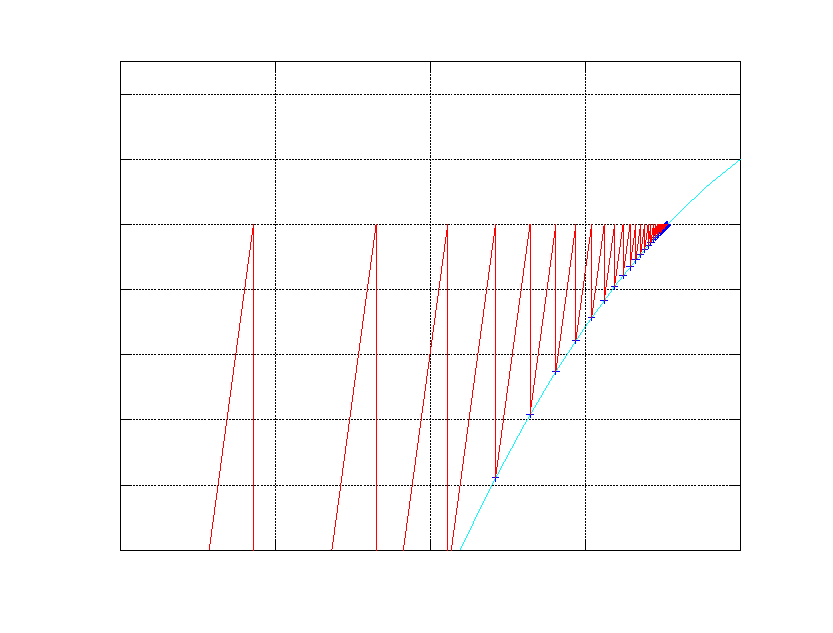
\includegraphics{RadiciEquazione/quasiNewton/chordNewtonRecursionNegativePlotOutput}}%
    \gplfronttext
  \end{picture}%
\endgroup

\end{center}
